%%%% ijcai22.tex

\typeout{A Practical Approach to Multi-Agent Path Finding in Robotic Warehouses}

% These are the instructions for authors for IJCAI-22.

\documentclass{article}
\pdfpagewidth=8.5in
\pdfpageheight=11in
% The file ijcai22.sty is NOT the same as previous years'
\usepackage{ijcai22}

% Use the postscript times font!
\usepackage{times}
\usepackage{soul}
\usepackage{url}
\usepackage[hidelinks]{hyperref}
\usepackage[utf8]{inputenc}
\usepackage[small]{caption}
\usepackage{graphicx}
\usepackage{amsmath}
\usepackage{amsthm}
\usepackage{booktabs}
\usepackage{algorithm}
\usepackage{algorithmic}
\urlstyle{same}

% the following package is optional:
%\usepackage{latexsym}

% See https://www.overleaf.com/learn/latex/theorems_and_proofs
% for a nice explanation of how to define new theorems, but keep
% in mind that the amsthm package is already included in this
% template and that you must *not* alter the styling.
\newtheorem{example}{Example}
\newtheorem{theorem}{Theorem}

% PDF Info Is REQUIRED.
% Please **do not** include Title and Author information
\pdfinfo{
/TemplateVersion (IJCAI.2022.0)
}

\title{A Practical Approach to Multi-Agent Path Finding in Robotic Warehouses}

% Single author syntax
\iffalse
\author{
    Submission \#11
    % \affiliations
    % The 2nd International Workshop on Heuristic Search in Industry
    % \emails
    % 
}
\fi

% Multiple author syntax (remove the single-author syntax above and the \iffalse ... \fi here)
\iftrue
\author{
\mbox{Jonathan Morag$^{1,2}$}\and
\mbox{Ariel Felner$^1$\and}
\mbox{Roni Stern$^1$\and}
\mbox{Dor Atzmon$^1$\and}
\mbox{Eli Boyarski$^1$\and}
\mbox{Sria Louis$^2$\And}
\mbox{Meir Toledano$^2$}
\affiliations
$^1$Ben-Gurion University of the Negev\\
$^2$Get Fabric, Inc.\\
\emails
moragj@post.bgu.ac.il,
felner@bgu.ac.il,
\{sternron, dorat, boyarske\}@post.bgu.ac.il,
\mbox{\{sria.louis, meir.toledano\}@getfabric.com}
}

\fi


\usepackage{float}
\usepackage[]{todonotes}
% \usepackage[disable]{todonotes}
\usepackage{xspace}
\newcommand{\benchone}{Benchmark1\xspace}
\newcommand{\benchtwo}{Benchmark2\xspace}
\newcommand{\soc}{SOC\xspace}
\newcommand{\sr}{Subset Reroute\xspace}
\newcommand{\allA}{All Agents\xspace}
\newcommand{\manA}{Mandatory Agents\xspace}
\newcommand{\freeA}{Free-space Conflicting Agents\xspace}
\newcommand{\len}{len\xspace}
\newcommand{\mkspn}{makespan\xspace}
\newcommand{\lm}{Lifelong MAPF\xspace}
\newcommand{\avgthr}{Average Throughput\xspace}
\newcommand{\indthr}{Average Individual Throughput\xspace}
\newcommand{\timeto}{Time to X\% Completion\xspace}
\newcommand{\thrat}{Throughput at t\xspace}
\newcommand{\ad}{Agent Density\xspace}
\newcommand{\tuple}[1]{\ensuremath{\left \langle #1 \right \rangle }}

\newcommand{\citet}[1]{\citeauthor{#1}~\shortcite{#1}}


\begin{document}

\maketitle

\begin{abstract}
    \begin{small}
    Multi-Agent Path Finding (MAPF) is a challenging problem that has recently been the subject of both theoretical research in academia, and practical application in industry. Many works extend MAPF definitions and algorithms to encompass different aspects of real use-cases, or improve different aspects of an algorithm's performance. However, many of these works are applied on academic environments. Thus, they are not easily combined with each other and applying them to real world settings are not trivial.
    In this work we review some of the challenges of applying MAPF algorithms to robotic warehouses, present our approach to meeting those challenges and suggest a framework for solving MAPF problems in this application. This includes solving a lifelong version of MAPF. We also suggest several useful metrics for comparing algorithms in this problem and how they change as agent density increases. In our experiments we show that prioritized planning is very effective in such environments despite its simplicity.
    \end{small}
\end{abstract}

\section{Introduction}

Multi-agent Path Finding (MAPF) is the problem of finding a set of non-conflicting paths for a set of agents on a graph. MAPF has recently received significant interest in many research works \cite{stern2019multi,felner2017search}. MAPF is relevant for several existing and emerging practical applications, such as robotic warehouses, UAV deliveries, airport routing, and autonomous vehicles \cite{ma2019lifelong,ho2019pre,li2019departure,dresner2008multiagent}. Different applications of MAPF require various modification over the classical definitions of MAPF, and it is not always clear or easy to modify existing MAPF algorithms accordingly. 

In this work, we discuss in details two main challenges that arise when implementing MAPF solutions for a practical application in an automated robotic warehouse. The challenges are: implementation cost and evaluation metrics. These challenges are in fact the focus of our main research questions that arise in our joint work with a commercial company that operates robotic warehouses.

\noindent \textbf{Implementation Cost.} 
In many real world cases the benefit of using more sophisticated MAPF algorithms may be outweighed by the human efforts in building and maintaining them. 
We therefore propose that simple MAPF algorithms may be more valuable than previously thought. They provide solutions of reasonable quality, while also being simple to implement and modify for real use-cases. 
To this end we provide an empirical evaluation comparing simple MAPF algorithms to a more sophisticated state of the art MAPF algorithm. We perform this evaluation on two types of MAPF problems: classical MAPF and \emph{\lm}, which is an online variant of MAPF where the agents are given a sequence of path planning tasks to perform. 
\lm is an important variant as it has real-world application when routing multiple robots in a robotic warehouse. 

For classical MAPF, we explore the usefulness of \emph{Prioritised Planning} \cite{latombe1991multiple} (PrP), a simple and widely-used MAPF algorithm, and evaluate the benefit of using it over more sophisticated MAPF algorithms. Our results show that PrP with a simple modification --- using random restarts --- often yield comparable results to an optimal MAPF algorithm (CBS), achieving average solutions whose quality was at most 11.5\% of optimal in our experiments. For \lm, we show that employing PrP with restarts under a framework we call \emph{\sr}, can improve the solution quality and problem coverage of existing algorithms. 

\noindent \textbf{Evaluation Metrics.} 
Finding the appropriate metrics to compare MAPF solutions and demonstrate their usefulness is key to effectively using them in the real world. We introduce new metrics with which to compare \lm solutions. We then compare these metrics with existing metrics. 
These metrics, which we call \emph{\indthr}, \emph{\timeto}, and \emph{\thrat}, are meant to evaluate the throughput of the solution in terms of reaching many goals quickly. \indthr measures the average throughput per agent. \timeto measures the time taken to reach some percent of all goals. \thrat measures the number of goals reached within a given time window.
Appropriate metrics are also useful for making application design decisions. We show this by examining an aspect of \lm, that is not typically covered by MAPF research -- finding the number of agents that should be used in a MAPF system to achieve the best average throughput or success rate~\cite{salzman2020research}. In this examination we see that the gain in throughput achieved by our solver remains fairly steady, with a mild decreasing trend. By contrast, its coverage does eventually begin to decrease rapidly, but only after more than 100 agents are added.


\section{Definitions and Background}

In the Multi-Agent Path Finding (MAPF) problem, the input is a graph $G=(V,E)$, and a set $A$ of agents, where each agent $a_i$ is associated with a pair of source and goal vertices $(s_i \in V,g_i \in V)$. A path $p$ is a sequence of vertices such that each vertex is connected to the successive vertex by an edge (called a move action), or the successive vertex is the same vertex (called a wait action) ($\forall t | ( (p[t], p[t+1]) \in E ) \lor ( p[t] = p[t+1] )$). Two paths $p_i, p_j$ are said to conflict if two agents following them would occupy the same vertex at the same time, or swap their vertices in one move ($\exists t | p_i[t] = p_j[t] \lor (p_i[t] = p_j[t+1] \land p_i[t+1] = p_j[t])$).
A \emph{solution} to the MAPF problem is a mapping $\pi$ of each agent $a_i\in A$ to a path $p_i$ that starts at its source and ends at its goal, such that no two paths conflict. 
The length of a path is defined as the number of vertices (non-unique) in the path, minus one ($\len(p) = |p| - 1$). A cost function $\mathit{cost}$ maps a solution to a numeric cost. \emph{Sum Of Costs} (\soc) is a common cost function for MAPF, defined as the sum of the lengths of all plans in the solution ($\soc(\pi) = \sum (\len(p) | p \in \pi)$). Another well known cost function is \emph{Makespan}, defined as the maximum length amongst all paths in the the solution ($\mkspn(\pi) = \max(\len(p) | p\in \pi)$). A solution is considered \emph{optimal} by some cost function if it is has the minimum cost of all solutions to a MAPF problem.

\emph{Prioritised Planning} (PrP) \cite{latombe1991multiple} is a simple and well known planning technique, which was also adapted for solving MAPF problems~\cite{silver2005cooperative}. In PrP, the agents are sorted by some (often arbitrary) priority ordering. Then, individual paths are computed for the agents in order of their priority, where each agent avoids the paths of all higher priority agents. PrP is incomplete and sub-optimal, but it is fast (polynomial in the number of agents) and very simple to understand, implement, and extend. 

A simple and effective improvement to PrP is \emph{Prioritised Planning with Random Restarts} (PrPr). In PrPr, several iterations of PrP are performed. For each iteration, a different random priority ordering is used. The best solution found during those iterations is returned. This procedure increases the running time linearly while improving the quality of the solution and increasing the likelihood that any solution will be found.

PrP and PrPr are often used in MAPF research as a baseline \cite{ma2019searching,andreychuk2018two}.

\emph{Conflict Based Search} (CBS) is an optimal MAPF solver. CBS performs a best-first search according to solution cost on a binary tree called the \emph{constraint tree} (CT). This is called the high-level search. The CT is initiated with a root node, containing a solution, where individual paths are created for each agent while ignoring all other agents. These paths are created using a single-agent search algorithm, referred to as the low-level search. This solution may contain conflicts between the paths of different agents. 
% A conflict is a tuple $\tuple{a_i,a_j,v,t}$ where the paths of agents $a_i$ and $a_j$ collide at vertex $v$ at time $t$. 
CBS resolves these conflicts by constraining agents, thus limiting the actions they are allowed to make. A constraint is a tuple $\tuple{a_i,x,t}$ such that $a_i$ is an agent that is prohibited from occupying vertex $x$ at time $t$ if $x$ is a vertex, or prohibited from moving on edge $x$ between times $t-1$ and $t$ if $x$ is an edge. Every time a node in the CT is expanded, a conflict is chosen and two constraints are created, one for each agent in the conflict. Two child nodes are then created, one for each constraint, and the solution in each node is updated to satisfy the node's constraint. The child nodes are then inserted to OPEN. CBS halts when a node with no conflicts is chosen for expansion.


\section{Robotic Warehouses}

We are interested in the MAPF use-case of navigation within robotic warehouses. This use-case for MAPF has been gaining in prevalence in the industry and as a subject of MAPF research \cite{ma2019lifelong}. In a robotic warehouse, a team of robots (agents) must collaborate in order to move items within the warehouse or in and out of the warehouse (typically through dedicated locations at the edges of the map). 

\subsection{\lm}

As a MAPF problem, the missions that robots carry out in a robotic warehouse can be seen as abstract movement tasks (goals), scheduled and assigned online by some black-box assignment mechanism. We will refer to this modified MAPF problem as \emph{\lm}. The input to a \lm problem is a graph $G=(V,E)$ and a set $A$ of agents, where each agent $a_i$ is associated with a source vertex $s_i \in V$ and a queue $q_i$ of goal vertices. 
% In \lm, the MAPF problem is isolated from the assignment problem. To do so, tasks are pre-assigned and pre-scheduled. 
The queues are hidden, so that at any time, only the current goal is known for each agent. 
The solution to a \lm problem is a mapping $\pi$ of each agent $a_i\in A$ to a path $p_i$ that starts at its source $s_i\in V$ and passes through each one of its goals in the order that they appear in $q_i$, such that no two paths conflict. 
% This modification addresses a part of the Online Planning challenge explained above.

\subsection{Challenges in Robotic Warehouses}

The robotic warehouse use-case combines many characteristics that are not a part of the standard definition of MAPF. Thus, a MAPF implementation for this use-case would typically have to address at least some of the following challenges:

\textbf{Continuous Time and Space.} Classical MAPF assumes discrete timesteps and discrete locations in space. In the real world, actions may take non-uniform amounts of time, and the space that agents occupy (during movement or while stationary) can be continuous \cite{andreychuk2022multi,li2019multi,atzmon2020generalizing}. Concessions can be made to satisfy these assumptions. For example, all actions may be slowed such that they all take the same amount of time as the longest action. Similarly, the movement of agents may be limited such that the space is discretized. Such concessions come at the cost of the quality of solutions, and the system's robustness to imperfect execution. 

\textbf{Dense and Non-Standard Environments.} Grids are a typical environment used in MAPF. They are usually 4-connected, meaning that each cell is connected with its four adjacent cells with undirected edges, and all edges and actions have uniform (unit) costs \cite{stern2019multi}. Industrial applications may use grids as a base, but they may also have various application-specific constraints and considerations. This results in general graphs (not grids), non-unit costs, and intricate cost functions. These factors can cause bottlenecks, where certain parts of the graph are often densely populated.
Additionally, the source and goal locations of agents are typically assumed to be uniformly distributed. Real distributions of movement tasks may be heavily skewed towards certain goals or source-goal pairs. Again, this can cause areas of the graph to often be especially dense. A recent work modified an existing MAPF benchmark to reflect this~\cite{kaduri2021experimental}.

\textbf{Stochastic Actions.} The results of actions can never be guaranteed. They may be delayed or inaccurately executed, or they may depend on elements that are outside the scope of the MAPF system and whose service time is stochastic. This necessitates some consideration from the MAPF system, such as robust planning, or mitigation during execution 
\cite{atzmon2020robust,atzmon2020probabilistic}
% \cite{atzmon2020robust,atzmon2020probabilistic,shahar2021safe}
.

\textbf{Real-Time and Online Planning.} Most MAPF applications one can imagine require online planning that is constantly reacting to new requirements, changing environments, and execution errors \cite{ma2019lifelong,vsvancara2019online,atzmon2020robust,bogatarkan2019declarative}. 
Additionally, in such scenarios computation would have to happen in real-time, since it would be detrimental to pause the system until new paths are found \cite{li2021anytime}.
% time(-complexity) is money
Many MAPF algorithms are designed to find optimal solutions \cite{felner2017search}. These algorithms are often computationally demanding, but provide high quality (optimal) solutions. In the industry, it is often preferred that an algorithm will find a solution quickly even if it is (reasonably) sub-optimal, so long as it doesn't fail to find a solution when one exists. This issue is acknowledged and covered by several sub-optimal MAPF algorithms that provide different desired algorithmic characteristics such as being any-time, bounded-sub-optimal, or complete \cite{barer2014suboptimal}.

\textbf{Task Scheduling and Assignment.} Usually, movement tasks (goals) are given to specific agents, and those specific agents must be the ones to perform them (as soon as they are assigned). It is possible however to consider the assignment, and even the scheduling, of tasks to be part of the MAPF problem, allowing them to be optimized to improve the quality of solutions \cite{ma2019lifelong}.

% \textbf{Cost of Planning or Execution Failures.} The cost of failing to find a solution at any given time, or finding a solution that results in execution failures must be considered. Failures may cause local or global pauses, physical damage, delays, etc.

\textbf{Finding the Right Metric.} Different use-cases may have different priorities for the performance of their MAPF application. These can be affected by the characteristics of the use-case and by unique business considerations. As we show later in this paper, defining and choosing the right metric is not always straightforward.

% (work-)time is money
\textbf{Cost of Implementation Complexity.} We must consider the monetary cost of implementing complex algorithms. Even if it is possible to combine all the modifications necessary for a given MAPF application, and do so with a state of the art algorithm, such a system may be too complex to implement in a practical manner. A complex algorithmic solution requires both an upfront investment of development time, and an ongoing investment in the maintenance of the system. Additionally, a simple algorithm would be more flexible in accepting future modifications that were not considered when it was first implemented. For these reasons, the industry may prefer simple solutions and algorithms, even if they are lacking in many other aspects.

% intercompatibility (everything, everywhere, all at once)

While many of these characteristics have been considered in some form by existing works, each work typically only considers a single modification over the classic MAPF definition. Combining multiple modifications within the same system poses a serious challenge in and of itself. While it should theoretically be possible to combine many of existing algorithmic modifications, such intricate work is left to the system implementer. 
This problem is exacerbated when the plethora of different MAPF algorithms and their improvements are considered. Not every modification has been considered for compatibility with every algorithm. Even when a modification is considered for a particular MAPF algorithm, it is often not considered for compatibility with its state of the art improvements. 
% For example, any improvement that assumes MAPF is done on a grid \cite{li2019symmetry,harabor2011online} would not work if MAPF has to be done on a general graph.


\section{Evaluating \lm Solvers}

The metrics with which solutions are evaluated are used to inform design decisions. It is therefore very important to design the correct metrics for any MAPF application. 
% We examine which metrics are appropriate for evaluating \lm solvers, and then 
The metric of minimizing \soc or \mkspn, may be inadequate for \lm, as the primary concern should be finishing many tasks (arriving at goals) quickly, which these metrics do not directly measure. Additionally, it is important to note that towards the end of the solution, agents begin to deplete their goal queues, so performance during those timesteps is less indicative of the quality of the solution. Therefore, metrics should attempt to capture the steady-state of the the system. We also measure coverage (number of instances where any solution was found), since often failing to find a solution can be detrimental to the performance of a practical MAPF application.

We define the following metrics, specifically designed for the \lm problem:

\emph{\timeto} (lower is better) - The number of timesteps that passed until a percent $X$ or more of the total number of goals was achieved. We set this percent to be 50\%, to capture the steady-state of the system. This metric is relatively stable, as it can be used without special consideration with different maps, distributions, and numbers of agents or goals per agent. However, it hides the actual number of goals completed. For example, adding more agents may seem like it hurts performance since agents would interfere with each other, while in reality the throughput would increase since more agents would mean more goals are being worked towards simultaneously.

\emph{\avgthr } (higher is better) \cite{li2020lifelong} - The average number of goals achieved per timestep, equivalent to the total number of tasks divided by \mkspn. This metric is straightforward, but may be excessively influenced by a few (or even one) outlier agents with very long plans.

\emph{\indthr} (higher is better) - The average number of goals each agent individually achieved per timestep in its plan, equivalent to the total number of tasks divided by \soc. We show this metric multiplied by a factor of 100, for the sake of readability. This metric diminishes the effect of agents depleting their queues at different times.

\emph{\thrat} (higher is better) - The number of tasks completed up to and including timestep $t$. We set this timestep to be 300, as agents usually (though not always) required more than 300 timesteps to deplete their queue of goals in this particular benchmark. This metric can clearly show the effect of using more agents on the velocity with which goals are completed. However, to capture the steady-state of the system, $t$ must be manually set according to the typical length of plans, which can vary by map and goal distributions, and the number of tasks each agent is given.

\section{The \sr Framework}

Next, we introduce \sr, a simple framework that can sufficiently satisfy the requirements of \lm. Additionally, we show how using simple algorithms within this framework can produce results that are close, or even superior to those achieved by more complex algorithms.

\sr is reminiscent of a lifelong equivalent of Large Neighborhood Search (LNS)~\cite{li2021anytime}. Unlike LNS, here the focus is not on optimizing a solution for an offline MAPF problem, but on efficiently solving many small MAPF problems as they arise in the process of solving \lm.
\sr is composed of three primary components: 

\textbf{(1)} \emph{Trigger} - Determines when to invoke a solver that might modify the existing solution. Here, we consider only one triggering option, where planning is only triggered when one or more agents require paths to new goals (have just reached their previous goals).

\textbf{(2)} \emph{Selector} - Selects a subset of the agents whose paths will be modifiable by the solver (other agents will be treated as mobile obstacles). We consider three methods for selecting agents:
\textbf{(a)}~\emph{\allA} always selects all agents. \textbf{(b)}~\emph{\manA} selects only agents that have no path to follow - i.e. agents who are at their goal (be it the last goal or one from the middle of the queue). These two methods are called PLAN-ALL and PLAN-NEW respectively, by \citet{ma2021competitive}. \textbf{(c)}~\emph{\freeA} selects all agents that \manA selects, but then also computes an individually optimal path for each of them (ignoring all other agents), and adds to the selection any agents whose current path interferes with any of the individually optimal paths.

\textbf{(3)} \emph{Sub-Solver} - Accepts the selected subset of the agents and the current solution, and computes a new solution while avoiding the paths of unselected agents. Most MAPF solvers may be modified to fit this purpose. We used CBS as an optimal solver, as well as PrP and PrPr with four restarts (PrPr4).

% \begin{table}[t] 
% \small
% \begin{tabular}{@{}lll@{}}
\toprule
                         & Selector               & Sub-Solver \\ \midrule
Snapshot Optimal         & All Agents             & CBS        \\
Mandatory Optimal        & Mandatory Agents       & CBS        \\
All Agents PrPr          & All Agents             & PrPr4      \\
Freespace Conflicts PrPr & Free-space Conflicting & PrPr4      \\
Mandatory Agents PrPr    & Mandatory Agents       & PrPr4      \\
Replan Single            & Mandatory Agents       & PrP        \\ \bottomrule
\end{tabular}
% \caption{Solvers created using \sr}
% \label{tbl:solvers}
% \end{table}

From these options we form six solvers 
% (summarized in table~\ref{tbl:solvers})
: 

\emph{Snapshot Optimal} (SO) \cite{stern2019multi} uses \allA and CBS. 
\emph{Mandatory Optimal} (MO) uses \manA and CBS. 
\emph{All Agents PrPr} (APR) uses \allA and PrPr4.
\emph{Freespace Conflicts PrPr} (FPR) uses \freeA and PrPr4.
\emph{Mandatory Agents PrPr} (MPR) uses \manA and PrPr4.
\emph{Replan Single} (RS) \cite{stern2019multi} uses \manA and PrP. 

\section{\ad}

The problem of \ad demonstrates one way in which metrics are used in informing the design of a MAPF system. When the aim is to maximize the throughput of a system, more agents initially translate into a higher throughput. However, space is finite and agents interfere with each other, so naturally the average individual throughput of agents decreases as more agents are added into the same space. Eventually, each additional agent would only hurt the total throughput. As an extreme example, imagine a large graph where all vertices are occupied. Any move would have to involve many agents moving in a synchronous manner and likely in a manner that is detrimental to the achievement of most of their individual goals. Surely, removing some of the agents would alleviate the congestion and increase the total throughput. It may therefore be beneficial to find the number of agents for a given map, where peak throughput is likely to be achieved~\cite{salzman2020research}. 

A simple way to estimate the best amount of agents is to experiment with different amounts of agents on different instances, and find where, on average, the quality or coverage are highest. For this purpose, selecting an appropriate metric is important.


\section{Experimental Results}

\begin{table*}[t] 
\small
\centering
\begin{tabular}{lllrrrrrrr}
\toprule
            &    &    &      SOC & Makespan & TimeTo50\% & AvgThrough & IndvThrough & Through@300 & Solved \\
Map Name & Agents & Solver &          &          &           &            &             &             &        \\
\midrule
Warehouse\_1 & 25 & SO &  9,997.30 &   537.30 &    235.10 &       0.47 &        2.50 &      161.20 &     11 \\
            &    & MO & 10,144.30 &   542.50 &    237.60 &       0.46 &        2.47 &      158.50 &     30 \\
            &    & APR & 10,186.50 &   539.50 &    236.10 &       0.47 &        2.46 &      160.90 &     49 \\
            &    & FPR & 10,002.80 &   538.20 &    235.60 &       0.47 &        2.50 &      161.00 &     50 \\
            &    & MPR & 10,154.10 &   543.70 &    237.40 &       0.46 &        2.46 &      158.90 &     50 \\
            &    & RS & 10,532.10 &   544.60 &    239.50 &       0.46 &        2.37 &      157.60 &     50 \\
            \hline
Warehouse\_2 & 30 & SO & 13,779.69 &   668.46 &    270.69 &       0.45 &        2.18 &      166.23 &     14 \\
            &    & MO & 13,934.15 &   669.92 &    275.15 &       0.45 &        2.16 &      164.31 &     26 \\
            &    & APR & 14,079.08 &   669.46 &    272.15 &       0.45 &        2.13 &      165.46 &     42 \\
            &    & FPR & 13,887.69 &   669.46 &    271.54 &       0.45 &        2.16 &      166.00 &     50 \\
            &    & MPR & 14,066.08 &   671.08 &    277.38 &       0.45 &        2.14 &      163.23 &     50 \\
            &    & RS & 14,658.08 &   671.15 &    277.92 &       0.45 &        2.05 &      162.85 &     49 \\
            \hline
Warehouse\_3 & 20 & SO &  8,000.00 &   569.40 &    242.10 &       0.36 &        2.51 &      126.10 &     10 \\
            &    & MO &  8,126.80 &   578.60 &    245.40 &       0.35 &        2.47 &      124.30 &     39 \\
            &    & APR &  8,239.40 &   571.60 &    243.30 &       0.35 &        2.43 &      125.10 &     46 \\
            &    & FPR &  8,046.20 &   571.60 &    242.30 &       0.35 &        2.49 &      125.40 &     50 \\
            &    & MPR &  8,215.90 &   575.30 &    247.30 &       0.35 &        2.44 &      122.70 &     50 \\
            &    & RS &  8,607.80 &   582.90 &    246.60 &       0.35 &        2.33 &      122.50 &     49 \\
\bottomrule
\end{tabular}

\caption{Comparison of different \sr versions}
\label{tbl:sr}
\end{table*}

PrPr is much easier to implement and extend than many other MAPF algorithms, such as CBS. Consequently, in this experimental section we aim to answer the following research questions: 
\textbf{(1)} What is the benefit, in terms of solution quality, of using CBS over PrPr. 
\textbf{(2)} What is the benefit in terms of the number of problems the system is able to solve (coverage / success rate), of using CBS over PrPr.

\subsection{Benchmarks and Experimental Setup}

We used maps and instances from two MAPF benchmarks:

\textbf{\benchone} is a standard MAPF benchmark \cite{stern2019multi}. In this benchmark, maps are 4-connected grids, and sources and goals are random, uniform, and non-repeating. We used 11 instances per map. From the maps in this benchmark, we used four empty grid maps of varying sizes.

\textbf{\benchtwo} is a set of warehouse maps and instances from a commercial company that jointly works with us on these matters. In this benchmark, maps are graphs whose connectivity is similar to that of 4-connected grids, and sources and goals were randomized based on the (skewed) distributions of real movement tasks in the warehouse. 
Therefore, some sources and some goals were assigned to more than one agent. In such events, agents that share the same source are allowed to jointly occupy it so long as they do so since the start of their paths. Equivalently, they are allowed to share their goal vertex at the ends of their paths. 
We used 50 instances per map.

For all following experiments where results for one map are compared across different number of agents, we filter instances per map in the following manner. 
% First, per amount of agents, we find all instances solved by all solvers on all agent amounts up to and including the current amount. Second, we choose the largest amount of agents where at least five instances were found. Finally, we keep only those instances found in the first step for the agent amount chosen in the second step. The end result is that all instances used were solved on all agent amounts and by all solvers, and that at least five such instances existed per map.
Only those instances solved by all numbers of agents and by all solvers were used, while the maximal number of agents was adjusted per map to ensure that a minimum of five instances are used in the final result.

All metrics were aggregated as averages. Coverage was aggregated as the sum of successful solution, and disregards the filtering of instances explained above.


\subsection{\lm Experiments}

For \lm, we experimented on maps and instances from \benchtwo, except that each agent was given a queue of nine goals (its source was unaffected). This queue was also generated using real distributions from each warehouse.

Table \ref{tbl:sr} shows the results of this experiment. Only the results for the largest number of agents per map are shown.
% Per map, we picked the highest amount of agents where at least five instances were solved by all solvers, and included only those instances. Results are aggregated as averages. 
Generally, across all metrics, the relation between solvers regarding the quality of their solutions was as follows: SO $>$ FPR $>$ APR $>$ MO $>$ MPR $>$ RS. It is interesting to note that \soc is particularly inadequate for this problem. The same applies for \indthr, since it is linearly related to \soc. As an example, we see that considering \soc, APR was always worse (higher) than MPR. Had we only used \soc, we might think that MPR produced higher quality solutions. However, on all other metrics APR had higher quality solutions. This is likely due to the behaviour of agents after they have reached their last goal. Unlike MPR, APR is able to move those agents in order to shorten the paths of agents that are still working on their goals. This results in longer paths for many agents, and thus a higher \soc, but actually results in a higher quality solution, since more goals can be finished earlier. 

The relation in terms of the coverage achieved by the different solvers was: MPR / FPR $>$ RS $>$ APR $>$ MO $>$ SO. Generally, the heavier solvers that include many agents or use an optimal sub-solver had the worse coverage, because they were likely to run out of time. RS also failed occasionally, but because it failed to find a solution at all, while still having time left.

Interestingly, FPR outperformed not only MPR, but also APR, on all metrics, even though APR can move some agents that FPR can not. It also had better coverage than APR, though it was slightly lower than that of MPR (on more agents, not shown in table \ref{tbl:sr}). This likely means that FPR was able to focus its search effort on more relevant agents, thus finding better solutions and doing so faster.

This experiment shows that powerful and complex algorithms (CBS) do not necessarily serve a MAPF application any better than simple algorithms (PrPr). This is demonstrated by the fact that while SO found the highest quality solutions, APR and FPR found higher quality solutions than MO, and both MO and SO performed worse in terms of coverage.


\subsection{Offline MAPF Experiments}

\begin{figure}[t]
\centering
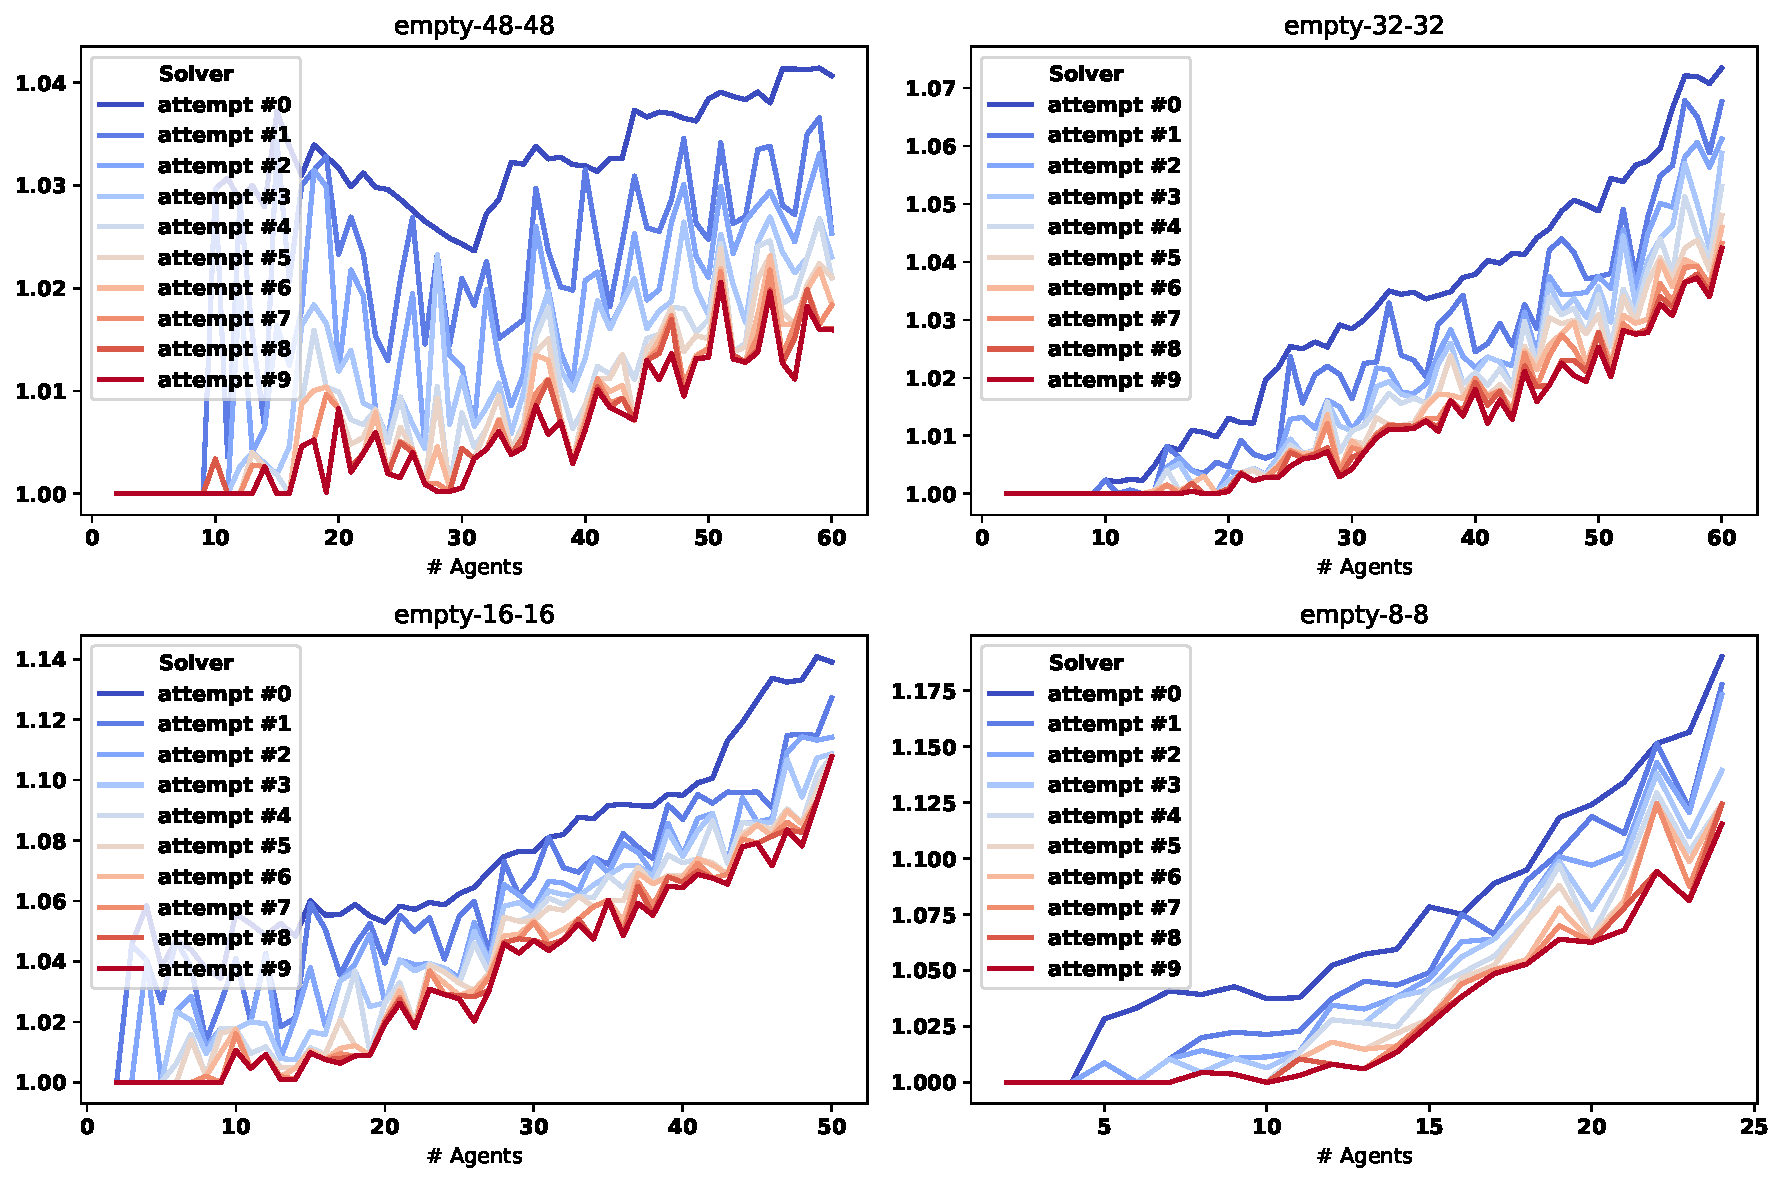
\includegraphics[width=\columnwidth]
    {figures/PrPr_vs_opt_empty.pdf}
    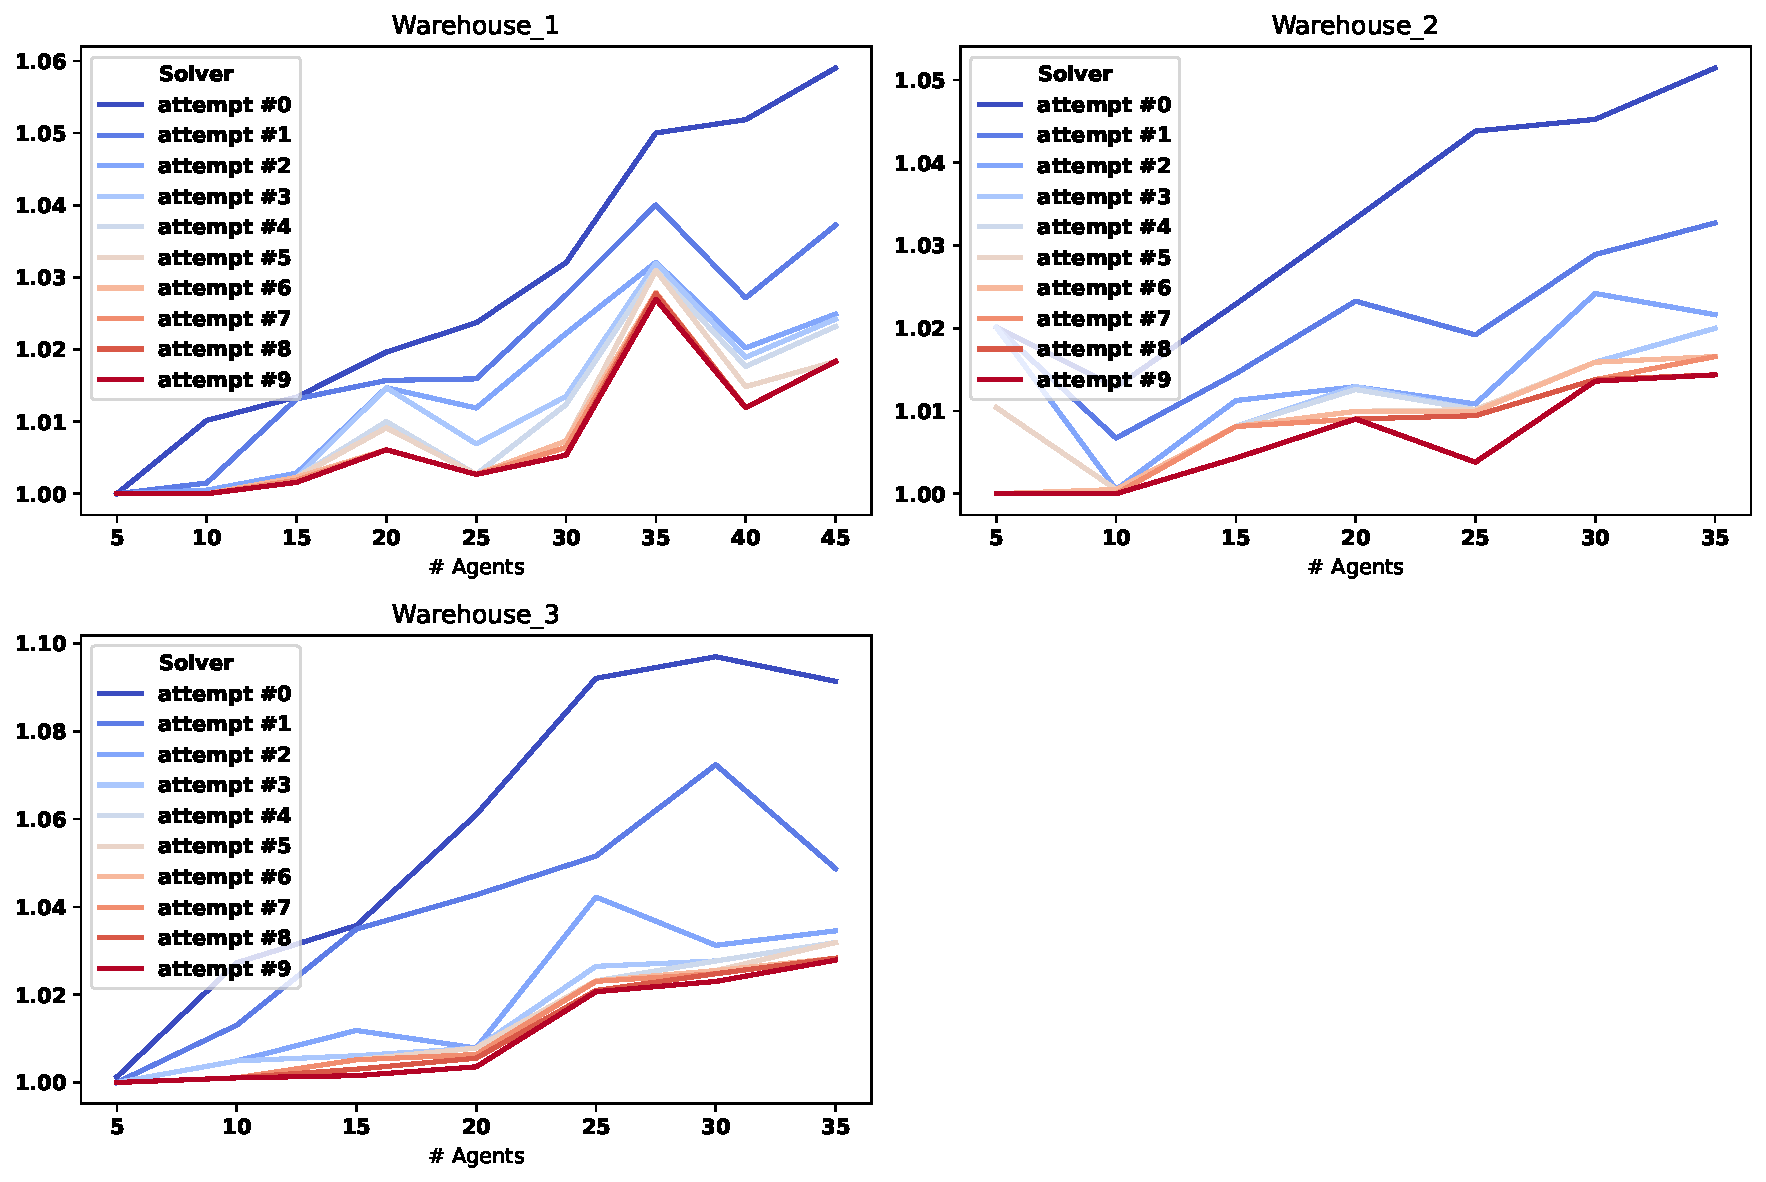
\includegraphics[width=\columnwidth]
    {figures/PrPr_vs_opt_warehouse.pdf}
\caption{\soc relative to optimal}
\label{fig:PrPr_vs_opt}
\end{figure}

To further reason about the results of our \lm experiment, we also compared the quality of solutions found by PrPr with those found by CBS (optimal solutions) in standard MAPF environments (\benchone) and under the standard definition of MAPF (offline).
The results of this experiment are shown in figure \ref{fig:PrPr_vs_opt} for seven different maps from both \benchone and \benchtwo. Each instance was solved by PrPr with nine restarts (10 total attempts), and the quality of the best solution found so far was recorded as the solution returned by each attempt (attempt \#0 is equivalent to PrP). The quality of the solutions is shown as a relative cost (\soc) compared with the cost of an optimal solution for the instance, found by a CBS \cite{sharon2015conflict} based optimal solver. The Y axis shows average relative \soc, and the X axis shows the number of agents. Note how this setup causes each iteration to always be better (lower) or equal to the previous iteration. Each solver was allowed 300 seconds to solve each instance, but the incomplete solvers may also fail earlier. 

Experiments on all sevens maps show a cost difference between PrP and optimal of a few percent with a few tens of agents. For example, on empty-16-16 with 40 agents, the difference was 9.5\% . There was a clear trend of the cost difference increasing as the number of agents increases. We observe that more dense maps produce a higher cost difference. This is true for the very small maps (like empty-8-8), but also for the warehouse maps, where the skewed goal distributions likely cause congested areas in the map where the density is high.
We also observe that a few random restarts significantly improve the quality of solutions (on average). However, the proportion of the improvement that is achieved decreases as the number of agents increases. For example, on map empty-16-16 with 30 agents, using nine restarts reduced the cost difference by 38.1\% (7.6\% to 4.7\%), but with 50 agents it reduced the difference by 23\% (13.9\% to 10.7\%). This may happen because as the number of agents increases
% , the number of possible priority orderings increases. Concurrently, 
the problem becomes more dense, so a larger proportion of the orderings results in low quality solutions or no solution at all. 
% Thus, restarts may help.
Additionally, we observe that most of the benefit of the random restarts can be gained by performing just a few of them, as the benefit gained from each additional restart seems to diminish quickly. This trend is to be expected. Since orderings are sampled completely randomly, the likelihood of finding an ordering that is better than the best one found so far decreases as more orderings are sampled.

% Additionally, we provide a comparison of the coverage (successful solutions) achieved by the different amounts of random \todo{ref table} restarts. In \benchone 11 instances were used per map, and in \benchtwo 50 instances were used per map.

These results demonstrate that despite its simplicity, PrPr can find solution whose quality is close to optimal.

\subsection{\ad Experiments}

\begin{figure}[t]
\centering
\includegraphics[width=\columnwidth]
% 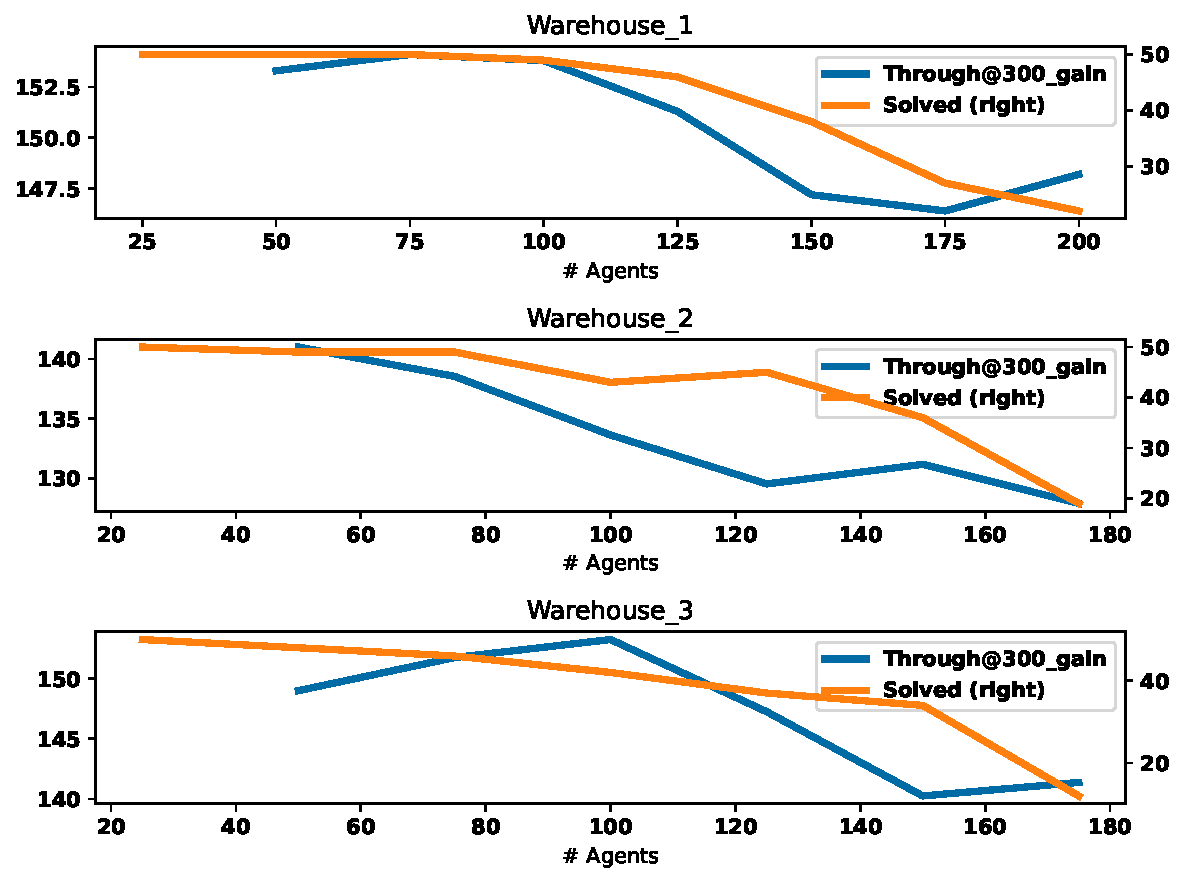
\includegraphics[width=\textwidth]
    {figures/mandatoryAgentsPrPr4_agents_density_throughputAtT250_performance.pdf}
\caption{Throughput gain and coverage by agent density}
\label{fig:agent_density}
\end{figure}

Figure \ref{fig:agent_density} shows the results of an \ad experiment, on the maps in \benchtwo. We used MPR because it had the best coverage in the \lm experiment. We used up to 200 agents per map. We show the coverage achieved per number of agents, before filtering instances (right Y axis). We show the gain in Throughput at 300 achieved by adding each batch of extra agents (left Y axis). We observe that the gain seems to decrease as more agents are added, but this trend is quite slow, as the gain was only reduced by about 10\% when the last 100 agents were added. Therefore, it is likely that many agents can still be added before they constrain each other's movements so often that throughput is reduced by adding them. This demonstrates that MPR can be quite powerful in terms of solution quality. On the other hand, coverage dropped much faster when more agents were added. Therefore, if a system has to contain hundreds of agents, it may be more important to optimize solvers for higher coverage, rather than solution quality. 
Regardless, we can learn from this experiment how many agents should be used by a system that uses MPR as its MAPF solver. For instance, if an average success rate of at least 80\% is desired, no more than 125 agents should be used on Warehouse\_2.



\section{Conclusions and Future Work}

We explored challenges and solutions in applying MAPF to real use-cases in the industry, particularly the robotic warehouse use-case (\lm). We showed that simple MAPF algorithms can achieve reasonable solution quality, while being easy to modify and extend. We also added new metrics by which to judge solutions for \lm. Finally, we explored the problem of Agent Density, where the goal it find how many agents should be used to improve throughput or achieve a high success rate.

Future work could explore other methods for the components of \sr, examine ways to avoid failing to find solutions under \sr, 
% find ways to convert failures to lower quality solutions so that both properties they could be evaluated as one metric, 
or find other ways to improve Prioritised Planning without making it more complex.


% \clearpage

% only on CAMERA READY
\section{Acknowledgements}

This research was sponsored by Get Fabric, Inc.
It was also sponsored by the United States-Israel Binational Science Foundation (BSF) under grant numbers 2017692 and 2021643, and by Israel Science Foundation (ISF) under grant number 844/17.
%% The file named.bst is a bibliography style file for BibTeX 0.99c
\bibliographystyle{named}
\bibliography{bibliography}

\end{document}



% application > challenges > lifelong > offline
%  metrics as challenge and contribution. 1. ease of implementation. 2. finding the right metric.
%  evaluating solvers in lifelong warehouse (before going into lifelonge xperiment). talk about metrics and also go into agents density. we show metrics and show a way to use it. metrics inform design choices. the framework works pretty well because the performance doesn't decrease dramatically.